\documentclass[a4paper,11pt]{article} %article style with 11pt fontsize
% \documentclass[fleqn,10pt]{olplainarticle}
% Use option lineno for line numbers 

\usepackage[utf8]{inputenc} %to add symbols like accents
\usepackage{graphicx} % to add figures
\usepackage{amsmath} % to add math and equation environments
\usepackage[margin=3cm]{geometry} % to define the style of the page, margin of 3cm
\usepackage{multicol} %you might need to do multiple columns
\usepackage{hyperref} %to create hyperlinks within the document
\title{Updated assessment of ${\Delta^{14}CO_{2}}$ measurement intercomparability using atmospheric records and standard materials}
\author{Christian Blair Lewis$^{1}$, Jocelyn Turnbull$^{1,2}$, Rachel Corran$^{1}$}
\date{\today}



\begin{document}

\maketitle

\pagenumbering{arabic} % arabic style (page numbering) for the rest of the document
\include{Abstract} 
\include{Intro}
\include{Method}
\include{Results}
\include{Conclusions}

\section{Supplementary Information}
\label{sec:conc}
\begin{figure}[h!]
  \caption{ Intercomparison of ${\Delta^{14}CO_{2}}$ measurements  at Cape Grim, Tasmania (CGO), and Baring Head, New Zealand (BHD) collected by NIWA and measured at Rafter Radiocarbon Laboratory. Dates represent the middle of the sampling period, which differ no more than one day between sites. These data show that during the time in which data are available, no measureable difference is found between the two sites. This provides some evidence that the two sites may be considered equivalent for this intercomparability study.}
% This data originally was sent to me in Jocelyn's first dropbox file. Later it was condensed to the currnent file in the H: drive.  H:\Science\Datasets\CGOvBHD
  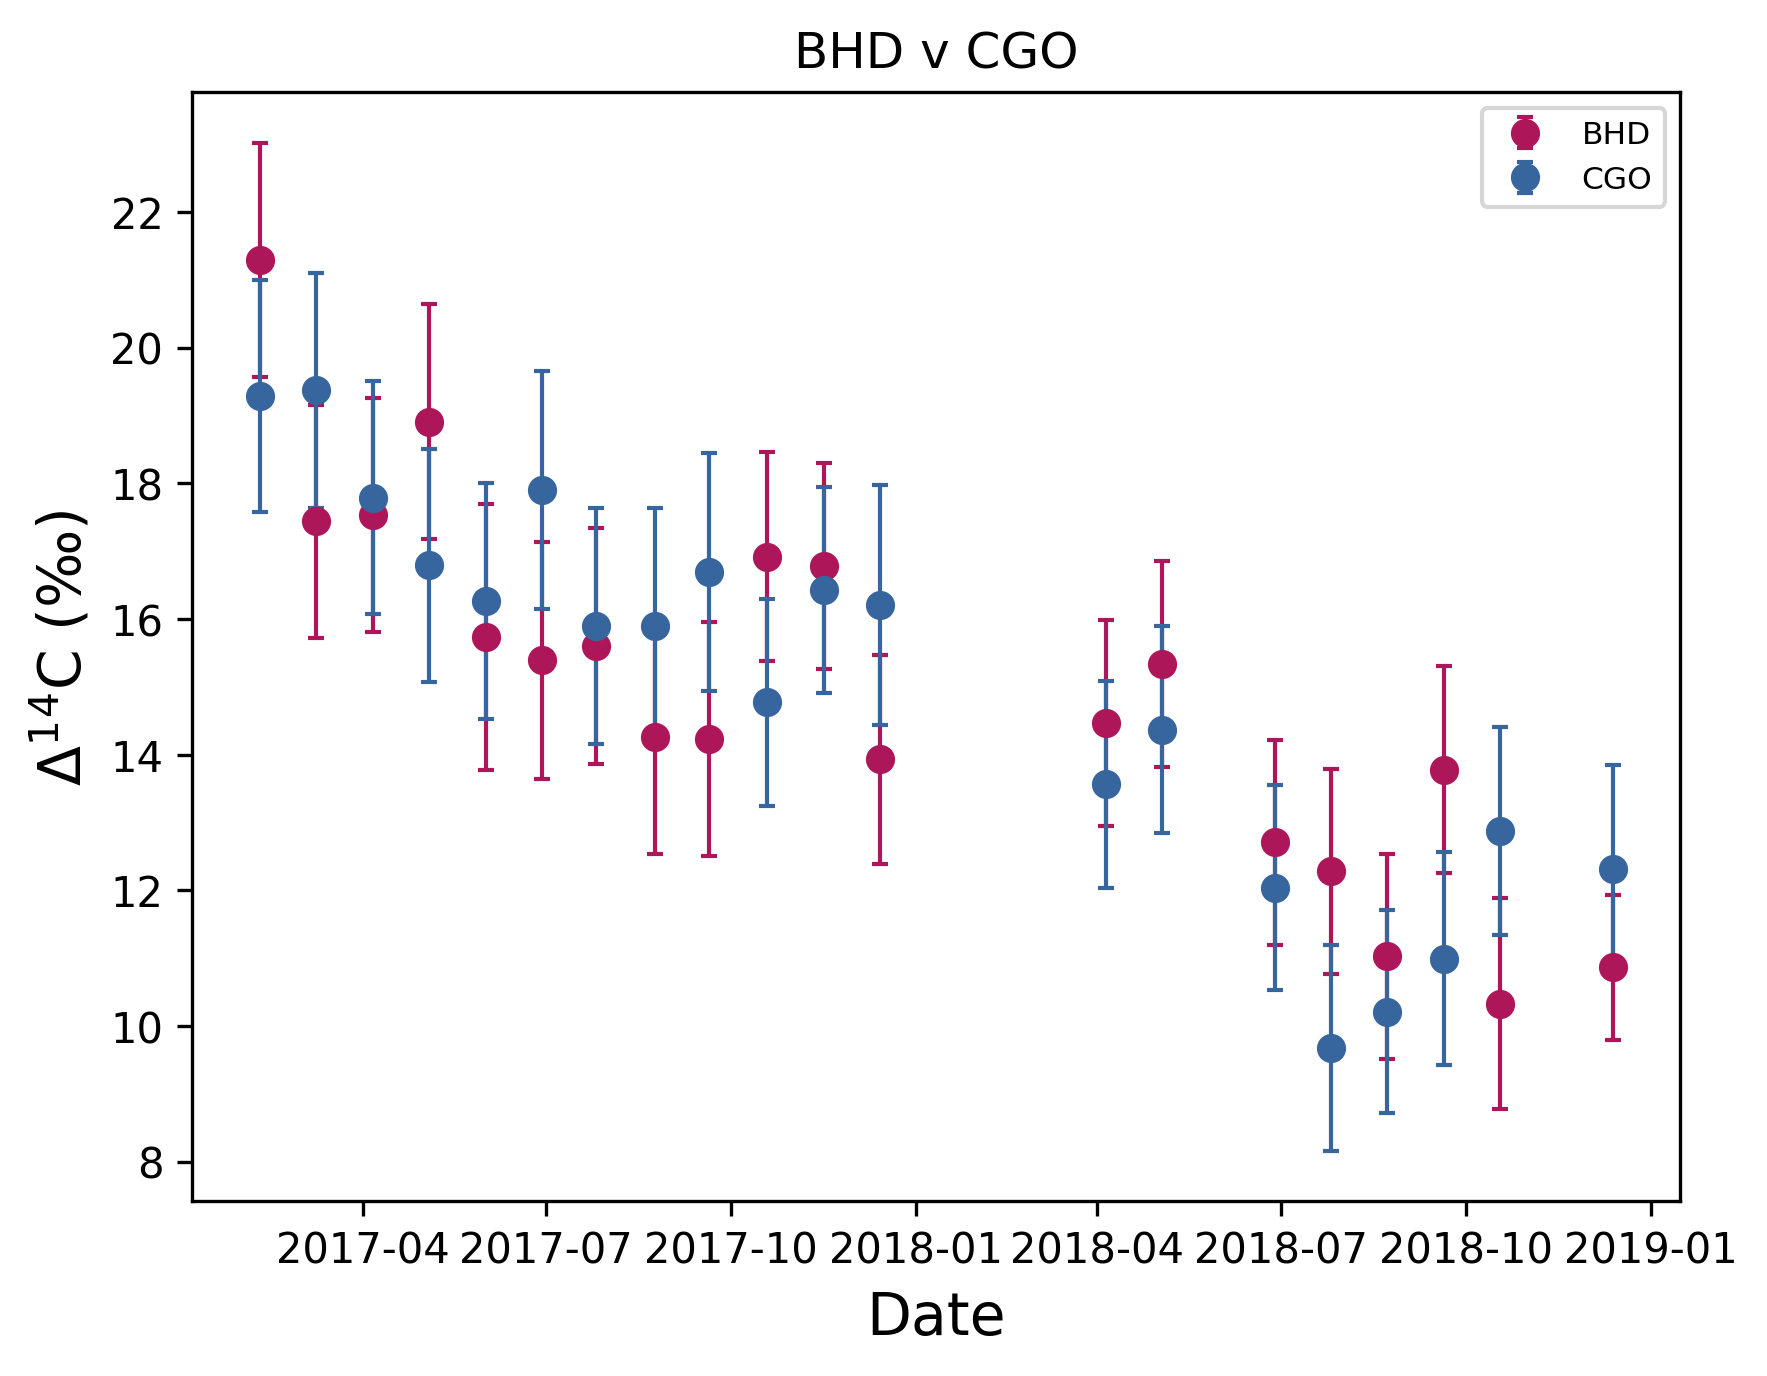
\includegraphics[width=1\textwidth]{/mnt/c/Users/clewis/IdeaProjects/GNS/Interlab_Comparison/output/Site_intercomparison.png}
\label{fig:bhdvcgo}
\end{figure}


\end{document}


% TODO: add a/b/c/d to figure 3 (the 8-panel plot of different trends/smooths)
% TODO: change one the lines in the above plot to be dashed or something so that if it's printed in black/white, its still recognizeable. 
% TODO: move the legend from the first Results figure (Heidelberg v RRL) 
% TODO: add a/b/c/d to the SIO LLNL plot as well
% TODO: remove the x-axis label from the top two panels of the SIO/LLNL plot
% TODO: replot all plots and make sure the colors / symbols are the same for each institution.
% TODO: change labels in b/d for SIo/lnl plots to SIO/LLNL
% TODO: change x-axis from "Date of Measurement" to Date.
% TODO: put ansto and magallanes plots next to each other, their so somolar and have similar results, this makes more sense. 

























